\documentclass[11pt,a4paper]{article}
\usepackage[a4paper,hmargin=1in,vmargin=1in]{geometry}
\usepackage{pgfplots}
\pgfplotsset{compat=1.17}

\usepackage[british]{babel}
\usepackage[utf8]{inputenc}
\usepackage[T1]{fontenc}

\usepackage{stddoc}
\usepackage{lipsum}
\usepackage{subcaption}

\newcommand{\plus}{{\texttt{+}}}
\renewcommand{\Re}{\operatorname{Re}}
\renewcommand{\Im}{\operatorname{Im}}
\newcommand{\fourier}[3]{\mathcal{F}_{#1}\!\left[#2\right]\!\left(#3\right)}
\newcommand{\ifourier}[3]{\mathcal{F}^{-1}_{#1}\!\left[#2\right]\!\left(#3\right)}


\begin{document}

\pagenumbering{arabic}

% Header
\noindent\LARGE\textbf{B2M17ANT -- theory}\normalsize\\
\noindent\rule{12.5cm}{0.4pt}

\section{Linear (wire) antennas}
\begin{enumerate}
    \item \emph{Units of all quantities}\\
    $[E] = \mathrm V/\mathrm m$, $[H] = \mathrm A/\mathrm m$, $[Z] = \mathrm{\Omega}$, directivity and gain $[D] = [G] = \mathrm{dB}$, $[S] = \mathrm W/\mathrm m^2$

    \item \emph{What is the directivity of isotropic antenna (in linear scale and \emph{dBi})?}\\
    $D = 0 \;\mathrm{dBi} = 1$

    \item \emph{Describe antenna as a filter (in which domains does it filter) and a transformer of waves from guided to waves in free space.}\\
    Antenna behaves like a passive filter in both frequency and spatial domain. It transforms guided waves from a waveguide into radiates waves propagating in free space.

    \item \emph{When an antenna is electrically small and large (in terms of $ka$)? Give examples of such antennas.}\\
    An electrically small antenna is an antenna with $ka \in (0.5, 1)$, where $k = 2\pi/\lambda$ is the wave number. En example of an electrically small antenna is the antenna of Titanic: physical length of $50 \; \mathrm m$ with $f = 500 \; \mathrm{kHz}$.

    \item \emph{What characterizes a TEM transmission line (impedance and operation with frequency)? Sketch distribution of E and H in (a) coaxial line, (b) rectangular waveguide with TE10 mode, (c) microstrip line.}\\
    A truly TEM transmission line is non-disperive meaning that its parameters such as characteristic impedance and phase velocity don't change with frequency. Such TEM mode exists in a coaxial line on all frequencies or in a microstrip line (quasi-TEM) under a specified \emph{cut-off frequency}. In metallic waveguides such as a rectangular waveguide, TE/TM modes propagate above respective cut-off frequencies.
    \begin{figure}[!ht]
        \centering
    \begin{subfigure}{0.45\textwidth}
        \centering
        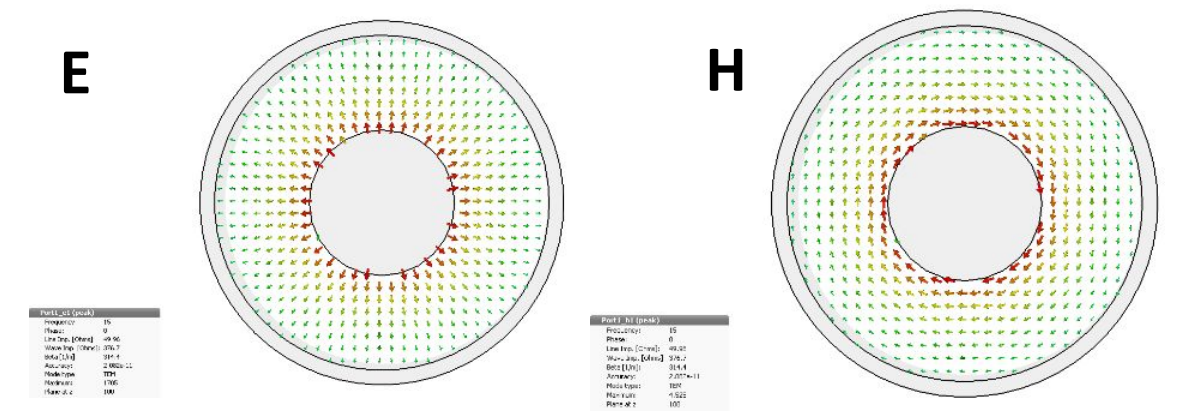
\includegraphics[width=\textwidth]{src/tem-coax.png}
        \caption{Coaxial TEM}
    \end{subfigure}
    \begin{subfigure}{0.45\textwidth}
        \centering
        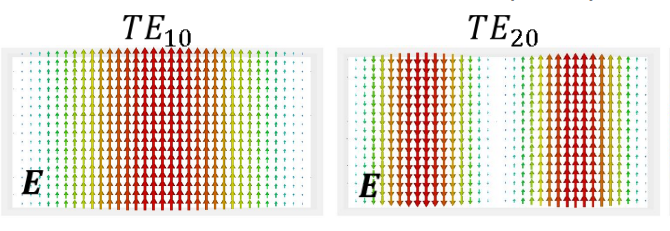
\includegraphics[width=\textwidth]{src/te-rectangular.png}
        \caption{Rectangular TE}
    \end{subfigure}\\
    \begin{subfigure}{0.9\textwidth}
        \centering
        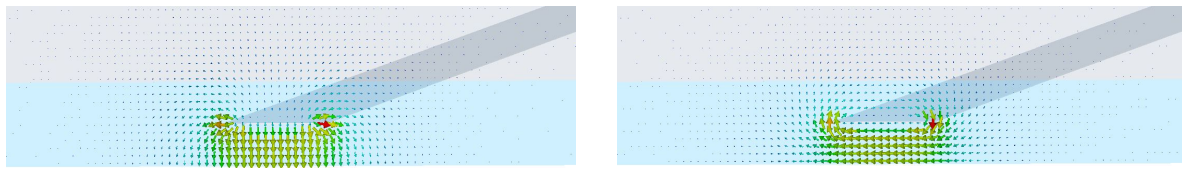
\includegraphics[width=\textwidth]{src/tem-microstrip.png}
        \caption{Microstrip TEM}
    \end{subfigure}
    \caption{\label{fig:propagation-modes}Propagation modes in different transmission lines}
    \end{figure}

    \item \emph{Sketch circuit model of a transmitting and receiving antenna.}\\
    See figure~\ref{fig:circuit-model-transmitting}.
    \begin{figure}[!ht]
        \centering
        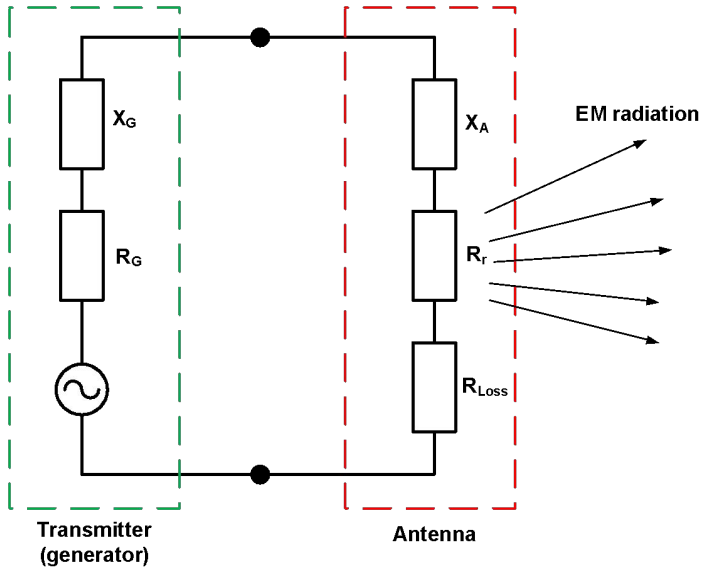
\includegraphics[width=0.6\textwidth]{src/circuit-model-transmitting.png}
        \caption{\label{fig:circuit-model-transmitting}Circuit model of a transmitting antenna}
    \end{figure}

    \item \emph{What is radiation resistance and radiation efficiency? Radiation efficiency of electrically small antennas.}\\
    Radiation resistance is the equivalent resistance accounting for the signal loss due to radiation.\\
    Radiation efficiency ($\eta = R_r/(R_r+R_{\mathrm{Loss}})$) is the ratio of the radiated power to the total power supplied to the antenna. Electrically small antennas tend to have small radiation efficiency.

    \item \emph{Define VSWR, Return Loss and relative bandwidth.}\\
    Voltage Standing Wave Ratio: $\mathrm{VSWR} = (1+|\Gamma|)/(1-|\Gamma|)$, where $\Gamma = (Z_L-Z_0)/(Z_L + Z_0)$ is the reflection coefficient.\\
    Return Loss: $\mathrm{RL} = -20\log_{10}|\Gamma|$ in dB.\\
    Relative bandwidth: $\mathrm{BW} = (f_2-f_1)/f_0 = (f_2-f_1)/\sqrt{f_1f_2}$.

    \item \emph{What is the physical meaning of the free space Green's function?}\\
    The free space Green's function corresponds to the one of a spherical wave.

    \item \emph{Elementary electric dipole -- what field components it does have (if z-oriented) in near and far field? What is its farfield pattern and why it is not isotropic even for dipole length approaching 0.}
    \begin{itemize}
        \item Near (reactive) field region $kr \ll 1$: Fields are similar to those of a static electric dipole and to the of a static current element. $E_r$ and $E_\theta$ are out-of-phase with $H_\varphi$. There is no time-average power flow nor radiated power; energy is stored in the near-zone.
        
        \item Intermediate field region $kr > 1$: Field are similar to those of a static electric dipole and to the of a static current element (quasistationary fields). $E_\theta$ and $H_\varphi$ approach time-phase which means the beginning of time-average power flow in the outward (radial) direciton.
        
        \item Farfield region $kr \gg 1$: Most important region of an antenna. $E_r$ vanishes and only transversal (to $r$) field components ($E_\theta$ and $H_\varphi$) remain.
    \end{itemize}
    It can't be isotropic even for dipole length approaching 0 due to its farfield pattern $f(\theta,\varphi) = \sin(\theta)$. Magnetic dipole has farfield components $E_\varphi$ and $H_\theta$.

    \item \emph{Define radiation intensity and antenna directivity. Directivity vs electrical size of antenna. Radiation pattern properties (sidelobe level, front-to-back ratio, half power beamwidth, polarization).}\\
    Radiation intensity $U$ is defined as the power radiated from an antenna per unit space angle (in steradians) and is related to the farfield $E$ of the antenna:
    \begin{align*}
        U(\theta,\varphi) = r^2S(\theta,\varphi) = \frac{r^2}{2Z_0} \norm{E(\theta,\varphi)}^2.
    \end{align*}
    Directivity is the ratio of the radiation intensity in a given direction from the antenna to the radiation intensity averaged over all directions, i.e., isotropic source:
    \begin{align*}
        D(\theta,\varphi) = \frac{U(\theta,\varphi)}{U_0} = \frac{4\pi U(\theta,\varphi)}{P_r}.
    \end{align*}
    Maximum directivity is then given by
    \begin{align*}
        D_{\mathrm{max}} = \frac{U_{\mathrm{max}}}{U_0} = \frac{4\pi}{\oint_S f_n^2(\theta,\varphi) \; \d S}.
    \end{align*}
    For example for the elementary electric dipole, $f_n(\theta,\varphi) = \sin(\theta)$ and $D_{\mathrm{max}} = 3/2$ in linear scale which corresponds to $10\log(3/2) \; \mathrm{dBi} \approx 1.76 \; \mathrm{dBi}$.\\
    Sidelobe level: radiation intensity level of the most significant sidelobes.\\
    Front-to-back ratio: power ratio of the main lobe to the back lobe.\\
    HPBW: bandwidth across which half of the power is radiated.\\
    Polarization is defined as the property of an EM wave describing the time-varying direction and relative magnitude of $\vec E$. Most common types are linear and circular (LHC/RHC).

    \item \emph{Can we speak about farfield if an antenna is embedded in an lossy space of infinite background?}\\
    We cannot since the radiation pattern is defined on a sphere with the radius approaching infinity. Thus it does not make sense to speak about it in a lossy environment.

    \item \emph{How to evaluate radiation resistance from radiation pattern and are there other possibilities?}\\
    One possibility is to integrate the Poynting vector $\vec S$ over a closed surface around the antenna to obtain the radiated power $P_r = I^2 R/2$ from which we can obtain the radiation resistance $R$.\\
    An alternate way is to calculate the radiated power $P_r$ using source currents instead of fields.

    \item \emph{What is EIRP?}\\
    EIRP stands for effective isotropic radiated power and it is the total power which must be radiated by an isotropic antenna in order for it to yield the same radiation intensity in a given direction. The units of EIRP are watts (W).

    \item \emph{Explain the physical meaning of the following integral:}
    \begin{align*}
        \vec A(\vec r) = \frac{\mu}{4\pi} \int_{V'} \vec J(\vec r') \frac{e^{-ikR}}{R} \; \d V'
    \end{align*}
    The integral states that the field vector potential is a sum of contributions in the form of source currents $\vec J$ multiplied by the Green's function of a spherical wave.

    \item \emph{Mark $r$ terms which contribute to near and far field. Which antenna does produce these fields? What is its orientation in cartesian cordinates?}
    \begin{align*}
        H_{\varphi}(r,\theta) &= \frac{ikIL}{4\pi} \sin(\theta) \bigg[ \underbrace{\frac 1r}_{\mathrm{farfield}} + \underbrace{\frac{1}{ikr^2}}_{\mathrm{nearfield}} \bigg] e^{-ikr},
    \\
        E_r(r,\theta) &= \frac{Z_0IL}{2\pi} \cos(\theta) \bigg[ \underbrace{\frac{1}{r^2}}_{\mathrm{nearfield}} + \underbrace{\frac{1}{ikr^3}}_{\mathrm{nearfield}} \bigg] e^{-ikr},
    \\
        E_\theta(r,\theta) &= \frac{ikZ_0IL}{4\pi} \sin(\theta) \bigg[ \underbrace{\frac 1r}_{\mathrm{farfield}} + \underbrace{\frac{1}{ikr^2}-\frac{1}{k^2r^3}}_{\mathrm{nearfield}} \bigg] e^{-ikr},
    \\
        H_r &= H_\theta = 0,
    \\
        E_\varphi &= 0.
    \end{align*}
    From simple vanishing properties of polynomials: only the terms of order $-1$ don't vanish in farfield. The above is the solution for the elementary electric dipole oriented in the $z$-axis and its length approaches 0.

    \item \emph{Current distribution on linear (wire) antenna, what approximations are used (constant, triangular and sinusoidal current)?}\\
    Assuming $z$-axis orientation (thin antenna), the distributions take form of
    \begin{align}
        \tag{Triangular}
        I(z) &= I_0\(1-\frac{2|z|}{L}\),
    \\
        \tag{Sinusoidal}
        I(z) &= I_0 \sin\(k\(\frac L2-|z|\)\).
    \end{align}
    For length $L = 0.5\lambda$, we obtain the sinusoidal distribution, the triangular distribution arises for smaller dipoles, and the constant distribution is the case of the elemental dipole.

    \item \emph{Sketch current distribution at dipoles of lengths $0.1\lambda$, $0.5\lambda$, $1\lambda$, $1.25\lambda$, $2\lambda$, \dots What effect do out-of-phase currents have on farfield?}
    \begin{figure}[!ht]
        \centering
        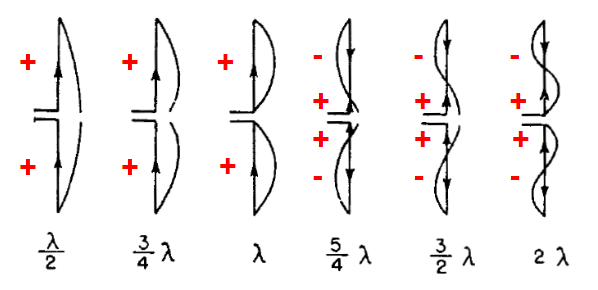
\includegraphics[width=0.8\textwidth]{src/dipole-lengths.png}
        \caption{\label{fig:dipole-lengths}Current distributions for different dipole lengths}
    \end{figure}
    Out-of-phase currents (caused by $L > \lambda$) produce sidelobes in the farfield.\\
    Missing distribution of $L = 0.1\lambda$: triangular distribution.

    \item \emph{Evaluation of near and far field of linear antennas -- far field approximation, Fourier transform between current and far field, polarization projections, \dots}\\
    The farfield approximation revolves around the expression
    \begin{align*}
        R \approx r-\Delta = r-z' \cos(\theta) = r-\vec r' \cdot \vec e_r.
    \end{align*}
    The $\Delta$ term's contribution can then be neglected in amplitude but not in phase. This approximation leads to the useful conclusion that the radiated field is directly proportional to the Fourier transform of the source currents.

    \item \emph{Directivity of linear antennas ($1.25\lambda$ dipole)}
    \begin{figure}[!ht]
        \centering
        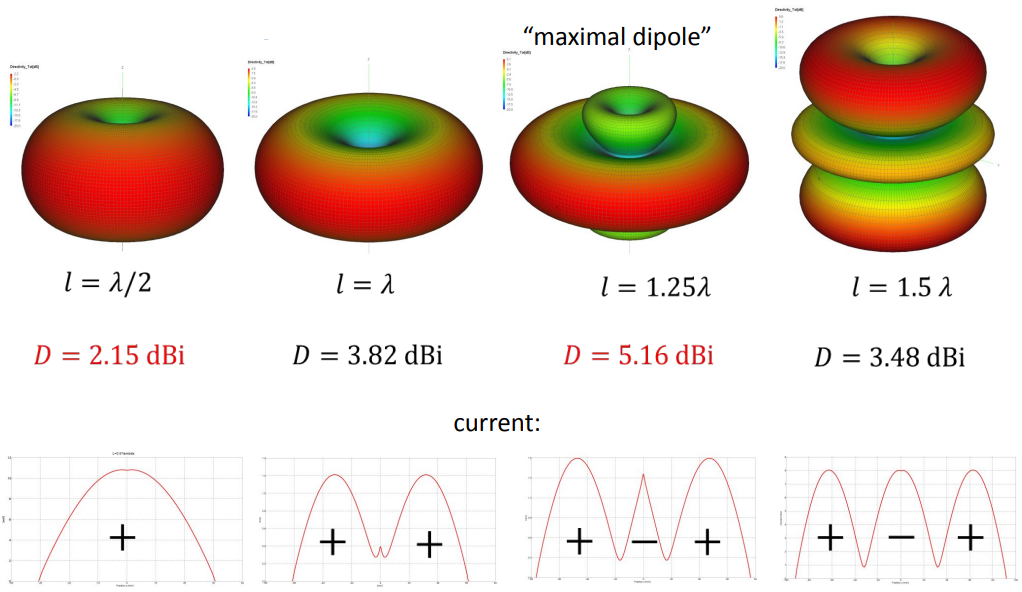
\includegraphics[width=0.8\textwidth]{src/dipole-radiation-patterns.png}
        \caption{\label{fig:dipoles-radiation-patterns}Radiation patterns of dipoles}
    \end{figure}

    \item \emph{$\lambda/2$ dipole properties (input impedance, pattern), shortening to resonance, bandwidth}\\
    Radiation pattern: omnidirectional in the $H$-plane which is a useful property for many applications including mobile communications.\\
    Directivity: reasonable value (2.15 dBi), larger than of short dipoles.\\
    Imput impedance: $~73 \; \Omega$ which is pretty much well matched with a standard transmission line of characteristic impedance of $75 \; \Omega$; not sensitive to changes in the radius of the dipole.\\
    Shortening: the dipole itself is not exactly resonant and hence should be shortened by a little amount depending on the radius.\\
    Bandwidth: 5 to 15 \% from the central frequency depending on the input impedance.

    \item \emph{Folded $\lambda/2$ dipole -- impedance, pattern}\\
    Its impedance is about 4 times of the normal dipole which significantly increases its bandwidth. The pattern is similar to the normal dipole I think?

    \item \emph{Symmetrization, baluns}\\
    Symmetrization problem arises when connecting an unbalanced transmission line to the antenna. The balanced mode is when there are equal and opposite currents.\\
    Balun transforms the balanced input impedance of the dipole to the unbalanced impedance of the coaxial line such that there is no net curernt on the outer conductor of the coax.\\
    Further comments: non-symmetrical feeders are cheaper and simpler but require a symmetrization element (balun) for connection to the symmetrical antenna.

    \item \emph{Monopole antennas (impedance, pattern compared to dipoles), method of images}\\
    Impedance: roughly half the dipole version\\
    Gain: roughly double (+3 dBi)\\
    Pattern: radiates only above ground\\
    Method of images: mathematical replacement of the ideally infinite ground plane by a virtual opposite electrode creating dipole structure for radiation. In practice, we use radial lines (pieces of wires) instead of the ideal infinite ground plane.

    \item \emph{Horizontal dipole above ground -- method of images}\\
    By superposition, the ground plane above which the horizontal dipole sits can be modelled by a virtual image dipole with opposite current feed in the halfspace below ground plane.

    \item \emph{Explain what the terms in braces physically represent:}
    \begin{align*}
        E_\theta(r,\theta,\varphi) &= \underbrace{\frac{ikZ_0}{4\pi} \frac{e^{-ikr}}{r} \sin(\theta)}_A \underbrace{\int_{-l/2}^{l/2} I_z(z') e^{ikz' \cos(\theta)} \; \d z'}_B
    \end{align*}
    A: element factor (elementary dipole contribution)\\
    B: space factor (Fourier transform of the sources)
\end{enumerate}

\section{Aperture antennas}
\begin{enumerate}

    \item \emph{Aperture antennas -- equivalent source approach}\\
    First, we envelop the antenna with a closed surface because we are interested in the field far beyond the antenna, not the field nearby. Then we substitute the sources distributed inside the closed surface (`volume of the antenna') by sources only on the surface. These currents must be so that they produce the same field around the antenna. Lastly we set the fields inside equal to zero which alters the field inside where we don't care. 
    
    \item \emph{Aperture in infinite ground plane and in free space -- what equivalent sources to use?}\\
    Infinite ground plane: $\vec M = -2\vec n \times \vec E$.\\
    Free space: $\vec M = -\vec n \times \vec E$ and $\vec J = \vec n \times \vec H$. Additionally we demand that the feeding waveguide contains a TEM wave.
    
    \item \emph{Physical meaning of radiation integrals in near and far field. Far field distance, conditions for far field ($1/r$ dependence, $E/H$ ratio, transversal fields)}\\
    Aperture radiation can be imagined as the radiation of an infinite number of point sources placed in the aperture. The radiation integrals are a superposition of these sources' contributions.\\
    For nearfield, we need a numerical solution using original sources. Farfield described as distance greater than $2D^2/\lambda$, where $D$ is the maximal dimension of the antenna, allows for approximation which yields analytical solution. In farfield, impedance is equal to the impedance of the free space $Z = E/H = 120\pi \approx 377 \; \Omega$.
    
    \item \emph{Structure of the far field (Fourier transform $\times$ obliquity factors). Relation to array.}\\
    In farfield, the field can be expressed as the Fourier transform of the sources multiplied by obliquity factors, which include projection from Cartesian to spherical coordinates and a relation between $E$ and $H$.

    \item \emph{Huygens source properties, element factor.}\\
    Aperture antennas which can be considered Huygens sources have the virtue of perpendicular electric and magnetic fields. Furthermore:
    \begin{itemize}
        \item $E/H = Z_0 = 120\pi$,
        \item locally a plane wave,
        \item radiation pattern is a cardioid,
        \item element factor $(1+\cos(\theta))/2$.
    \end{itemize}

    \item \emph{Farfield of aperture with constant (amplitude, phase) source field}\\
    It can be expressed as a product of Fourier transforms of the source fields. Since constant source field means rectangular distribution, the far field is a product of sinc functions.

    \item \emph{Directivity of aperture antennas (effective area)}\\
    Directivity of aperture antennas can be easily computed using the effective area:
    \begin{align*}
        D_{\mathrm{max}} &= \frac{4\pi U_{\mathrm{max}}}{P_r} = \frac{4\pi}{\lambda^2}\frac{\left| \int_{S_A} \vec E_a(x',y') \; \d x' \d y' \right|^2}{\int_{S_A} \norm{\vec E_a(x',y')}^2 \; \d x' \d y'}
    \\
        &= \frac{4\pi}{\lambda^2} A_{\mathrm{eff}} = \frac{4\pi}{\lambda^2} \underbrace{A_{\mathrm{phys}}}_{A\cdot B}\underbrace{\eta_{\mathrm{amp}}}_{0.81}\underbrace{\eta^E_{\mathrm{phase}}(s)}_{0.8@s_{\mathrm{opt}}}\underbrace{\eta^H_{\mathrm{phase}}(t)}_{0.79@t_{\mathrm{opt}}}
    \end{align*}

    \item \emph{Sketch the field distribution in a rectangular waveguide with the TE10 mode. What is the amplitude and phase at its aperture?}
    \begin{figure}[!ht]
        \centering
        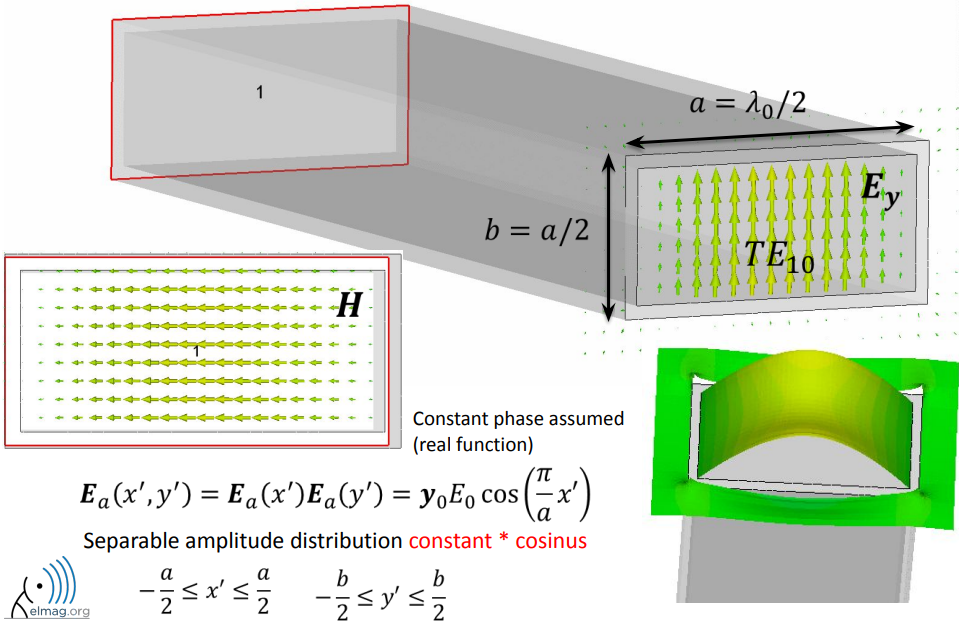
\includegraphics[width=.7\textwidth]{src/rectangular-waveguide-aperture.png}
        \caption{\label{fig:rectangular-waveguide-aperture}Rectangular waveguide in free space}
    \end{figure}

    \item \emph{Why does its radiation pattern differ in its $E$ and $H$ plane?}\\
    Because the field distribution in the aperture is different in each plane. One is constant (thus a sinc function field) and the other is a cosine (narrow field).

    \item \emph{1D aperture with linear and quadratic phase -- effects on pattern. Quadratic phase error -- where does it appear?}
    \begin{enumerate}[label=(\alph*)]
        \item linear phase variation: $\phi(x) \sim \beta x$
        \begin{itemize}
            \item HPBW increase
            \item directivity decrease
        \end{itemize}
        \item quadratic phase variation: $\phi(x) \sim \beta x^2$
        \begin{itemize}
            \item side-lobe levels rise
            \item minimums rise (filling zeros)
            \item loss in gain (widening of the main lobe)
            \item due to displacement of the reflector feed from focus, distortion of the reflector or lens, or a non-ideally-spherical wavefront of the feed, curved field in the aperture of a radiator
        \end{itemize}
    \end{enumerate}

    \item \emph{Polarization of aperture antennas}\\
    Decomposition of the radiated fields into co-polarization (intended to radiate) and cross-polarization (orthogonal to it). Highly dependent of the coordinate system: Ludwig-3 is the best because it gives the impression of polarization for aperture antennas and because it yields zero cross-polarization for Huygens sources.
    
    \item \emph{Horn antennas -- basic properties, why we use them and for what}
    \begin{itemize}
        \item Widening of a waveguide aperture, hence increase in gain
        \item low VSWR, fairly wide BW
        \item easy to manufacture/construct
        \item aperture efficiency of 50 to 80 \%
        \item primary feed for reflector antennas, radar, satellite, etc.
    \end{itemize}
    
    \item \emph{Phase effects in the aperture of a horn}
    \begin{figure}[!ht]
        \centering
        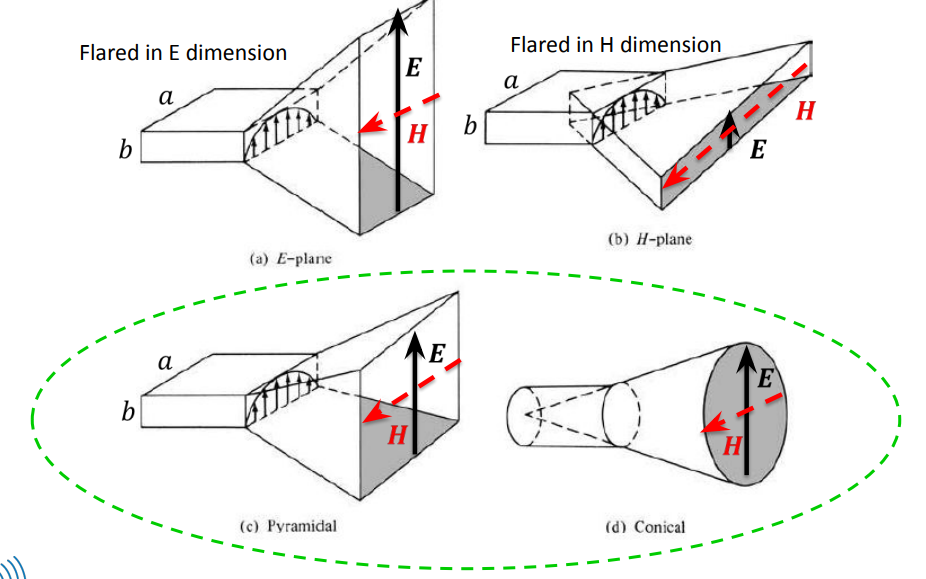
\includegraphics[width=.7\textwidth]{src/horn-antennas-types.png}
        \caption{\label{fig:horn-antennas-types}Types of horn antennas}
    \end{figure}
    
    \item \emph{Phase effects in the aperture of a horn}\\
    Due to the boundary conditions, electric field must be perpendicular to the slanted metal walls of the aperture, causing the field in the aperture to be slightly curved. This introduces a quadratic phase error, thus lower gain.

    \item \emph{Directivity vs aperture size (phase distortion), optimal horn, aperture efficiency}\\
    For a fixed axial length, the directivity increases by virtue of the increased aperture area. Optimum performance is reached for $t_{\mathrm{opt}} = 3/8$ which corresponds to a phase lag at the aperture edges of $\delta = 135^\circ$. Further increate beyond the optimum results in cancellations in the far field, thus a decrease in directivity.
    
    \item \emph{What is the phase center of a horn antenna}\\
    Apparent center of the spherical waves that emanate from the horn at a given radial distance, usually farfield. It is important for measurement and for reflector antennas -- phase center should always be aligned with the reflector focal point. For horns, the phase center is located inside the horn.
    
    \item \emph{Horns with mixed modes in aperture, why we do that. Polarization of horn antennas}\\
    Usually, we mix modes to obtain Huygens source, i.e., a source with no field curvature. Such a source produces a rotationally symmetrical radiation pattern which implies no cross-polarization.
    
    \item \emph{Explain the farfield approximation of the Green's function $\operatorname{exp}(-ikR)/R$ using figure~\ref{fig:farfield-approximation}:}
    \begin{figure}[!ht]
        \centering
        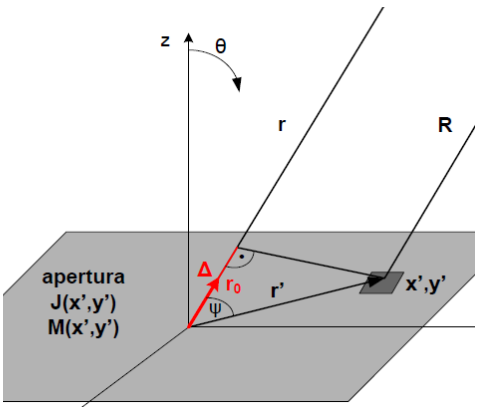
\includegraphics[width=0.5\textwidth]{src/farfield-approximation.png}
        \caption{\label{fig:farfield-approximation}Farfield approximation illustration}
    \end{figure}\\
    Using $R = r - \Delta = r - z'\cos(\theta)$, we can put
    \begin{align*}
        \frac{e^{-ikR}}{R} = \frac{e^{-ik(r-\Delta)}}{r-\Delta} \approx \frac{e^{-ikr}}{r}e^{ik\Delta}.
    \end{align*}
    The approximation is done assuming that $r \gg \Delta$ which means the resulting amplitude doesn't change much when we neglect the term in the denominator. However, doing this in the numerator would result in a huge error because phase is much more sensitive to small changes due to the behaviour of $\operatorname{exp}(ix)$. This approximation is the reason why we can use Fourier transform of the source currents to calculate farfield.
    
    \item \emph{What does the following integral describe and where is it used?}
    \begin{align*}
        \vec P(\theta,\varphi) &= \int_S \vec E_a(x',y') e^{ik(x'\sin(\theta)\cos(\varphi) + y'\sin(\theta)\sin(\varphi))} \; \d x' \d y'
    \end{align*}
    It is called the radiation vector and it is basically a Fourier transform of the aperture field. We can also regard it as a Huygens-like superposition of plane waves thanks to the exponential term.
    
    \item \emph{Explain all terms in the following equation. What does this equation represent?}
    \begin{align*}
        E_\theta(\theta,\varphi,r) &= \underbrace{\frac{iE_0ab}{\lambda}}_{\text{const.}} \underbrace{\frac{e^{-ikr}}{r}}_{\text{spherical wave}} \underbrace{\frac{1+\cos(\theta)}{2}}_{\text{obliquity factor}} \underbrace{\sin(\varphi)}_{\text{polarization projection}} \underbrace{\frac{\sin\(k_x \frac a2 \)}{k_x \frac a2} \frac{\sin\(k_y \frac b2 \)}{k_y \frac b2}}_{\text{FT of the source field}}
    \end{align*}
    This equation represents far field from an apreture with constant field in both dimensions (constant illumination).

    
    \item \emph{What does the graph in figure~\ref{fig:quadratic-phase-error-constant} describe?}\\
    It describes the impact of the quadratic phase error $\phi(x) = \beta (2/a)^2 x^2$. In the figure, $\beta = 0$ represents constant phase and $\beta = \phi/2$ represents a path length deviation of $\lambda/4$ from constant phase at the edges of the aperture.
    \begin{figure}[!ht]
        \centering
        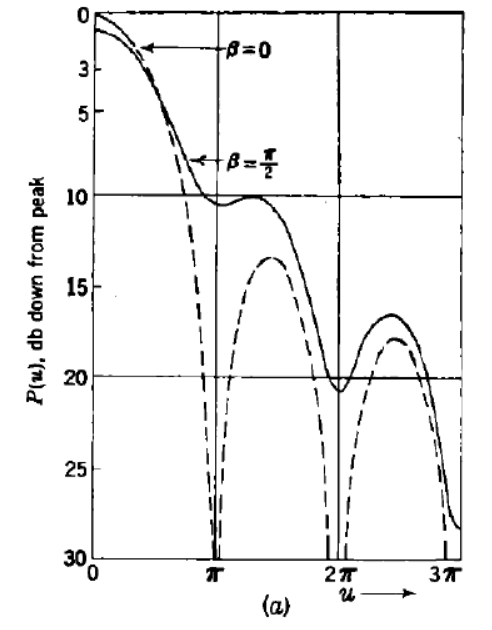
\includegraphics[width=0.4\textwidth]{src/what-is-this-graph.png}
        \caption{\label{fig:quadratic-phase-error-constant}Constant aperture illumination}
    \end{figure}
\end{enumerate}

\section{Reflector antennas}
\begin{enumerate}
    \item \emph{Why do we use the parabolic reflector antenna? What is its physical principle?}\\
    There are two big reasons to use parabolic reflector antennas: very high gain and a narrowly-directed beam with low sidelobe levels. The physical principle is that it transforms spherical wave into plane waves and vice versa.

    \item \emph{What happens if the feed is off the focus of a parabolic reflector antenna?}\\
    An offset causes phase errors which can slightly break the radiation pattern.
    
    \item \emph{Explain/sketch illumination and spillover loss in a parabolic reflector antenna.}\\
    See figure~\ref{fig:losses-in-reflector-antennas} for illustration. Illumination loss occurs because the feed's radiation pattern doesn't have a parabolic shape, hence the amplitude is not constant. Only a constant amplitude on the reflector would mean 100\% amplitude efficiency. Spillover loss is due to the fact that a part of the pattern `spills over' the reflector. An ideal feed (no illumination or spillover loss) cannot be fabricated because the goals contradict each other.
    \begin{figure}[!ht]
        \centering
        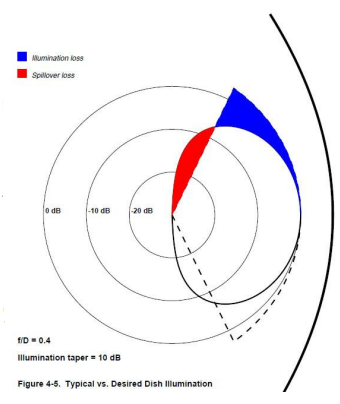
\includegraphics[width=.4\textwidth]{src/losses-in-reflector-antennas.png}
        \caption{\label{fig:losses-in-reflector-antennas}Illumination and spillover loss}
    \end{figure}
    
    \item \emph{What value of aperture efficiency is typical for the parabolic reflector antenna? What edge taper corresponds to the maximum efficiency?}\\
    Aperture efficiency 75 to 82 \%; optimal edge taper -11 dB.
    
    \item \emph{What are the properties of an `ideal' feed for a parabolic reflector antenna?}\\
    An ideal feed produces uniform amplitude and phase distribution which compensates for spherical spreading loss and doen't have spillover (cannot be made in practice). The feed should aim to accomplish the following goals:
    \begin{itemize}
        \item its pattern should be rotationally symmetrical (balanced feed);
        \item its pattern should be such that the reflector edge taper is -11 dB;
        \item have a point phase center located at the focal point of the reflector;
        \item be small in order to reduce blockage -- usually its diameter of the same order as wavelength;
        \item have low cross-polarization, usually below -30 dB.
    \end{itemize}
    
    \item \emph{What effects mostly contribute to an antenna's noise temperature?}\\
    Elevation angle, spillover.
    
\end{enumerate}

\section{Antenna arrays}
\begin{enumerate}
    \item \emph{Canonical arrays based on isotropic radiators, basic configurations, wavefront canceling, endfire/broadside arrays}\\
    The arrays are depicted in~\ref{fig:canonical-array-in-phase},~\ref{fig:canonical-array-out-of-phase}~and~\ref{fig:broadside-endfire}.
    \begin{figure}[!ht]
        \centering
        \begin{subfigure}{.45\textwidth}
            \centering
            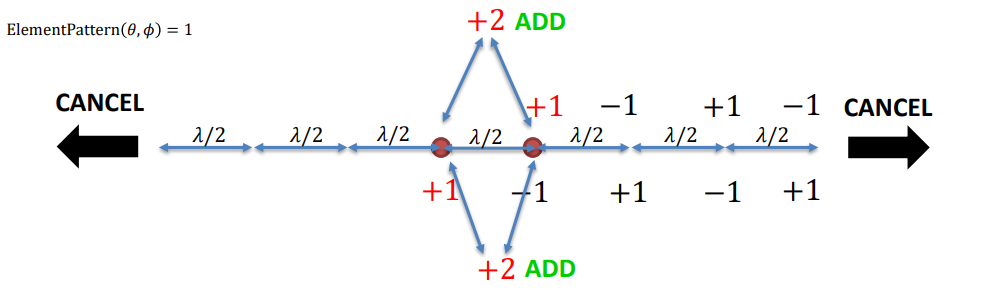
\includegraphics[width=\textwidth]{src/canonical-array-in-phase.png}
        \end{subfigure}\hfill
        \begin{subfigure}{.45\textwidth}
            \centering
            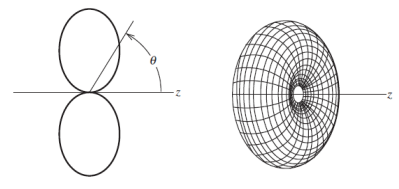
\includegraphics[width=\textwidth]{src/canonical-array-in-phase-pattern.png}
        \end{subfigure}
        \caption{\label{fig:canonical-array-in-phase}Canonical array with in-phase excitation}
    \end{figure}
    \begin{figure}[!ht]
        \centering
        \begin{subfigure}{.45\textwidth}
            \centering
            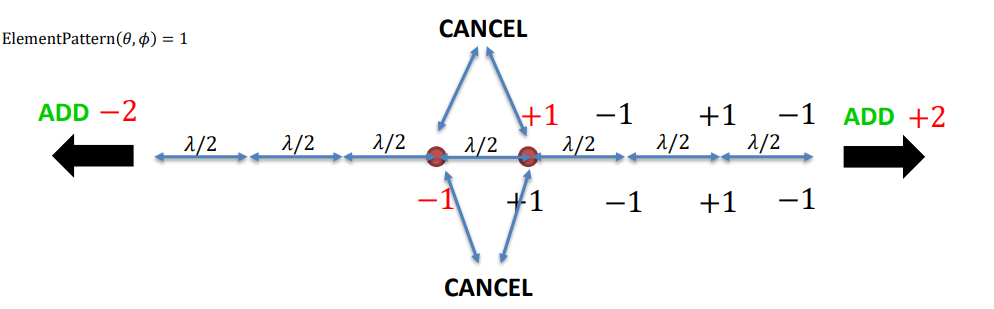
\includegraphics[width=\textwidth]{src/canonical-array-out-of-phase.png}
        \end{subfigure}\hfill
        \begin{subfigure}{.45\textwidth}
            \centering
            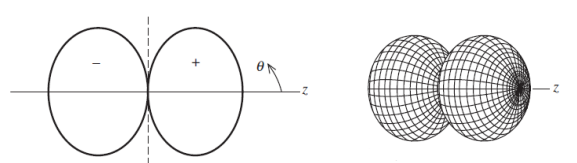
\includegraphics[width=\textwidth]{src/canonical-array-out-of-phase-pattern.png}
        \end{subfigure}
        \caption{\label{fig:canonical-array-out-of-phase}Canonical array with out-of-phase excitation}
    \end{figure}
    \begin{figure}[!ht]
        \centering
        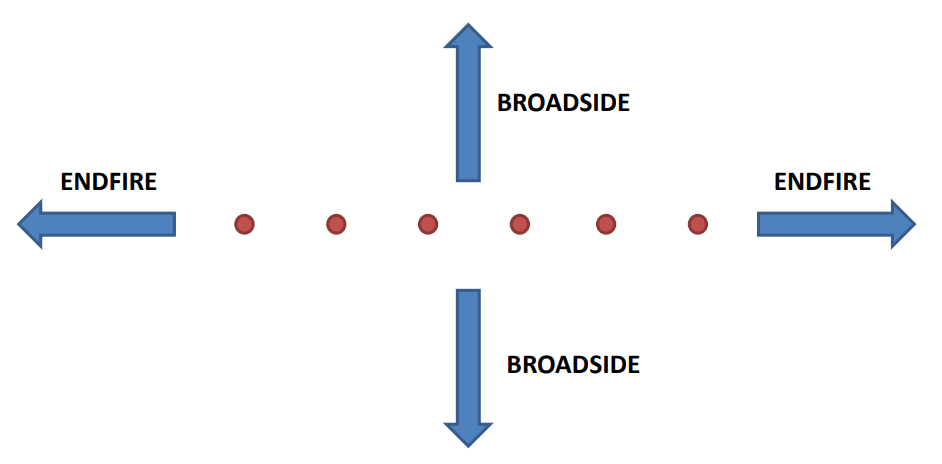
\includegraphics[width=.5\textwidth]{src/broadside-endfire.png}
        \caption{\label{fig:broadside-endfire}Broadside and endfire arrays}
    \end{figure}

    \item \emph{What is a canonical minimum scattering antenna, its importance in arrays. Element pattern, embedded pattern, array factor. Mutual coupling, mutual impedance.}\\
    Antennas with identical radiation patterns can differ in the manner and extent to which they modify an incident wave, i.e., in the way they scatter. A canonical minimum-scattering antenna (CSMA) is defined as one which becomes `invisible' when the accessible waveguide terminals are open-circuited. The scattering matrix of such an antenna is shown to be unique once N arbitrary orthogonal radiation patterns have been specified.\\
    Element pattern is the contribution of a single antenna in the array. It can be measured either isolated or embedded. Embedded means the antenna is placed in the array configuration with just one port excited and others terminated by 50 $\Omega$, i.e. isolated element pattern with scattering from the surrounding array.\\
    Array factor the other part of the total array radiation pattern. It is dependent on the geometry of the configuration. If we use minimum scattering antennas, the array radiation pattern is given as a product of the element pattern and the array factor.\\
    Mutual coupling represents the interaction of antennas in an array. Due to this effect, we define impedances
    \begin{align*}
        Z_{ij} &= \left.\frac{U_i}{I_j} \right|_{\forall k \neq j\,:\,I_k = 0}
    \end{align*}
    for $i,j \in \{1,2,\dots,N\}$ in an $N$-antenna array. Cases of $i=j$ correspond to so-called mutual impedances, whereas for $i \neq j$, we speak of mutual impedances. These make up the impedance matrix $\[Z_{ij}\]$. Additionally, it holds that $Z_{ij} = Z_{ji}$.
    
    \item \emph{Equally-spaced isotropic array -- properties, linear phasing}\\
    For general equally-spaced isotropic arrays, it holds that
    \begin{align*}
        AF = \sum_{n=0}^{N-1}I_n e^{iknd \cos(\theta)}.
    \end{align*}
    If the current has linear phase progression $I_n = A_n e^{in\alpha}$, we obtain
    \begin{align*}
        AF = \sum_{n=0}^{N-1}A_n e^{in\psi},
    \end{align*}
    where $\phi = kd\cos(\theta)+\alpha$. Furthermore, for a uniform array (same amplitudes $A_0$), we get
    \begin{align*}
        AF = A_0 e^{i(N-1)\psi/2} \frac{\sin\(N\psi/2\)}{\sin\(\psi/2\)}.
    \end{align*}
    Using this, we can tune the so-called scan angle $\theta_0$ and optimize $\alpha$ to obtain a broadside ($\theta_0 = \pm 90^\circ$, $\alpha = 0$) or an endfire ($\theta_0 \in \{0^\circ,180^\circ\}$, $\alpha = \pm kd$). Other options include the Hansen-Woodyard endfire array (increased directivity) or the Superdirective endfire array.
    
    \item \emph{Amplitude taper in arrays, its effect on pattern}\\
    More tapering towards the edges means more side lobe level reduction.
    
    \item \emph{Can be maximal directivity provided by a broadside or an endfire array?}\\
    Endfire arrays can reach more interesting values of directivity.
    
    \item \emph{Horizontal dipole above ground -- direcitivity, efficiency and impedance properties}
    \begin{itemize}
        \item Directivity: depends on the height of the dipole above ground,
        \item efficiency: bad,
        \item impedances: $Z_{11} = Z_{22}$, $Z_{12} = Z_{21}$, $Z_{\mathrm{in}} = Z_{11} - Z_{12}$.
    \end{itemize}
    
    \item \emph{Array directivity optimization, superdirectivity, sensitivity}\\
    Directivity optimization is done via tuning of the phase and amplitude distribution. Superdirectivity is very sensitive, thus it is imperative to have a precise feed.
    
    \item \emph{What does the following equation describe?}
    \begin{align*}
        AF = I_0 + I_1e^{ikd\cos(\theta)} + I_2e^{ik2d\cos(\theta)} + \cdots = \sum_{n=0}^{N-1} I_ne^{iknd\cos(\theta)}
    \end{align*}
    It describes the array factor of a general equally-spaced array of isotropic radiators.

    \item \emph{Sketch the element pattern, array factor and total pattern in the $xz$-plane for the following array:}
    \begin{figure}[!ht]
        \centering
        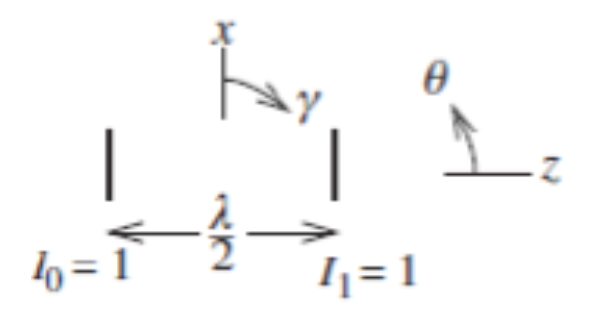
\includegraphics[width=.3\textwidth]{src/two-dipole-array.png}
        \caption{\label{fig:two-dipole-array}Array configuration}
    \end{figure}\\
    See figure~\ref{fig:two-dipole-array-pattern}
    \begin{figure}[!ht]
        \centering
        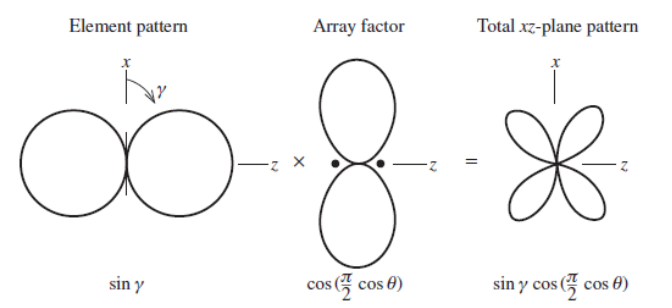
\includegraphics[width=.6\textwidth]{src/two-dipole-array-patterns.png}
        \caption{\label{fig:two-dipole-array-pattern}Array configuration patterns}
    \end{figure}

    \item \emph{Receiving antenna, circuit model}\\
    See figure~\ref{fig:circuit-model-receiving}
    \begin{figure}[!ht]
        \centering
        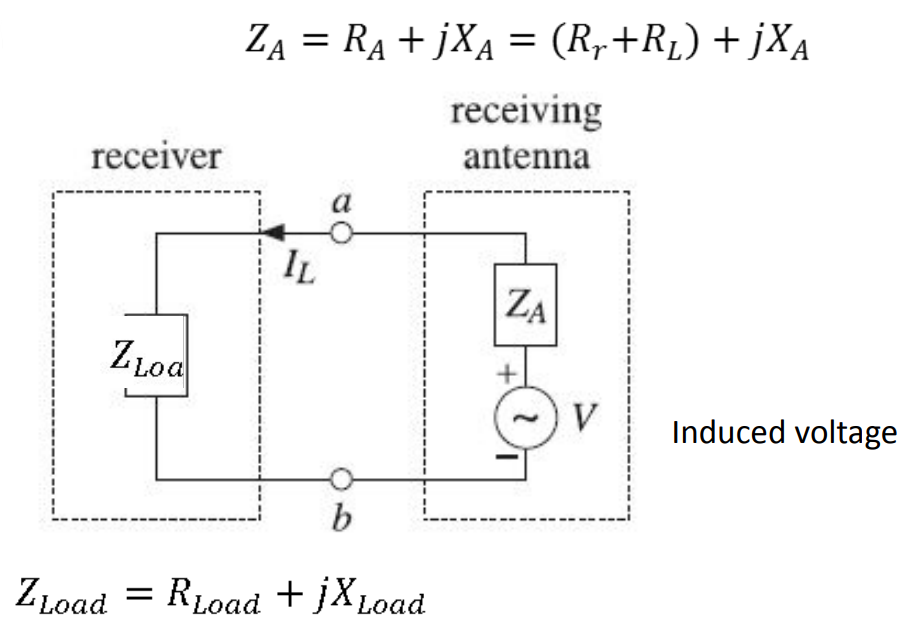
\includegraphics[width=.5\textwidth]{src/circuit-model-receiving.png}
        \caption{\label{fig:circuit-model-receiving}Circuit model of a receiving antenna}
    \end{figure}
    
    \item \emph{Effective length, effective aperture}\\
    Effective length: $U_{\mathrm{load}} = l_{\mathrm{eff}}E$.\\
    Effective area: $P_{\mathrm{load}} = A_{\mathrm{eff}} S_{\mathrm{inc}}$, boundary $A_{\mathrm{eff,max}} = (\lambda^2/4\pi)D_{\mathrm{max}}$.\\
    Both are virtual constructs for transforming incident quantity (electric field/power density) to load quantity (voltage/power).
    
    \item \emph{Effective aperture of the isotropic radiator and an antenna of arbitrary directivity $D$}\\
    Effective aperture of an antenna with arbitrary directivity is
    \begin{align*}
        A_{\mathrm{eff}} = \frac{\lambda^2}{4\pi}D
    \end{align*}
    which means that an isotropic radiator ($D=1$) is has the effective aperture of $\lambda^2/(4\pi)$.
    
    \item \emph{Friis' transmission equation}
    \begin{align*}
        P_{\mathrm{RX}} = P_{\mathrm{TX}}G_{\mathrm{TX}}G_{\mathrm{RX}}\(\frac{\lambda}{4\pi R}\)^2
    \end{align*}
    
    \item \emph{Explain what the following equation describes:}
    \begin{align*}
        S_{\mathrm{RX}} = \frac{P_{\mathrm{TX}}G_{\mathrm{TX}}}{4\pi R^2} \frac{\sigma}{4\pi R^2}.
    \end{align*}
    This is the radar equation and it expresses the power density of an echo signal received at the radar, reflected back from a target. Parameter $\sigma$ ($[\sigma] = m^2$) is the Radar Cross-Section (RCS) and it's a characteristic of the target as a measure of its size as seen by the radar.

    \item \emph{What is the difference between monostatic and bistatic radar?}\\
    See figure~\ref{fig:radar-types}.
    \begin{figure}[!ht]
        \centering
        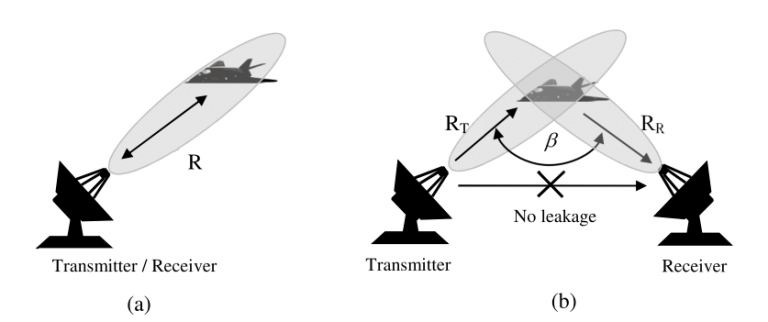
\includegraphics[width=.7\textwidth]{src/radar-types.png}
        \caption{\label{fig:radar-types}Monostatic and bistatic radar}
    \end{figure}
    
    \item \emph{Reciprocity theorem for antennas and its consequence for mutual impedances}\\
    Let us assume we apply voltage $V_a$ on antenna A and measure induced current $I_b$ on antenna B. Then we do the same vice versa: apply voltage $V_b$ on antenna B and measure induced current $I_a$ on antenna A. The reciprocity theorem for antenna states that if $V_a=V_b$, then $I_a=I_b$. As a consequence, $Z_{12}=Z_{21}$.
    
    \item \emph{Babinet's principle}\\
    An antenna has the exact same radiation pattern as its complementary structure which is the same configuration with `air and metal flipped', i.e. a slot in an infinite metal sheet of the same dimensions as the original antenna. An example of this duality is a dipole strip antenna and a slot antenna.
    
    \item \emph{Slot antenna vs strip dipole}\\
    Following from the Babinet's principle, their radiation pattern are ideally the same (practically not due to a finite metal sheet). However, the slot antenna has higher impedance. Furthermore, the ekvivalent circuit of a dipole is a serial RLC circuit, whereas for the slot antenna, its equivalent RLC circuit is parallel. They also differ in polarization.
    
    \item \emph{Slot antenna array based on rectangular waveguide}\\
    It is an array of fairly decent radiation efficiency. In a rectangular waveguide,%
        \footnote{The waveguide can be either fed from one side and shorted on the other or it can have both sides shorted and be fed from a input hole in the rear wall.}
    we create a standing wave which we then allow to radiate outside. The only source of radiation is the field in the slots which we can tune to set desired amplitude and reduce sidelobe levels. The slots are created in a zig-zag fashion in order to achieve in-phase pattern.
    
    \item \emph{Show the polarization and the radiation pattern in both planes of the antenna in figure~\ref{fig:slot-antenna}:}
    \begin{figure}[!ht]
        \centering
        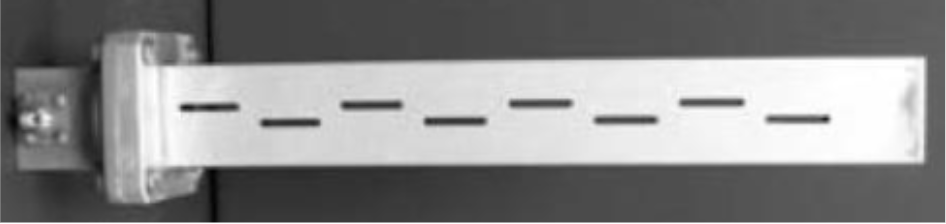
\includegraphics[width=.7\textwidth]{src/slot-antenna-array.png}
        \caption{\label{fig:slot-antenna}Slot antenna array}
    \end{figure}\\
    See figure~\ref{fig:slot-antenna-array}.
    \begin{figure}[!ht]
        \centering
        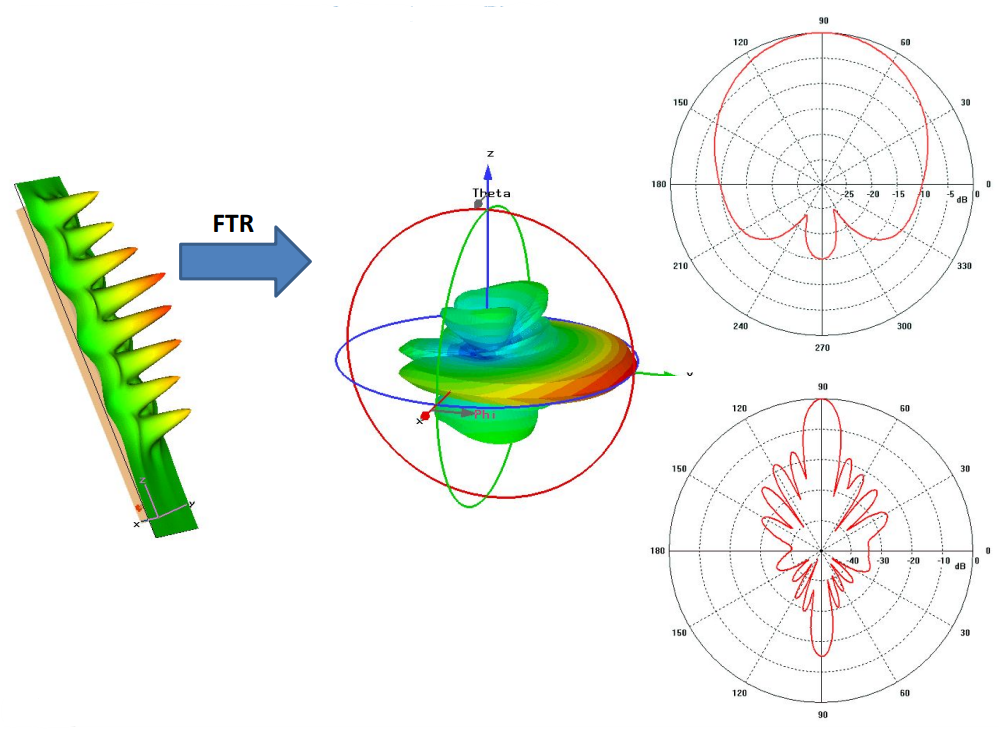
\includegraphics[width=.7\textwidth]{src/slot-antenna-array-patterns.png}
        \caption{\label{fig:slot-antenna-array}Slot anntenna array patterns}
    \end{figure}

    \item \emph{Rectangular microstrip antenna -- basic structure, field distribution, physical principle of radiation and }parameters\\
    Basic structure of rectangular microstrip antennas is identical to microstrip resonators except they are designed to radiate. Typical characteristics:
    \begin{itemize}
        \item incredible ease of manufacturing,
        \item moderate gain (7-9 dBi single element),
        \item usually low bandwidth due to its resonant nature,
        \item very good integration with a microwave circuit.
    \end{itemize}
    Radiation from a rectangular patch antenna can be modelled as of two slots in a metal plate which is equivalent to two parallel RLC circuits connected in parallel. The field distribution is illustrated in figure~\ref{fig:microstrip-field-distribution}.
    \begin{figure}[!ht]
        \centering
        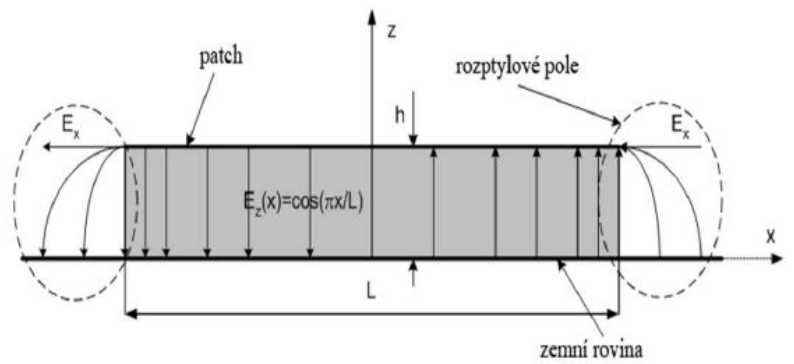
\includegraphics[width=.6\textwidth]{src/microstrip-field-distribution.png}
        \caption{\label{fig:microstrip-field-distribution}Patch antenna field distribution}
    \end{figure}
    
    \item \emph{Feeding of microstrip antennas for linear and circular polarization}\\
    The most common way to feed a microstrip antenna is by a coaxial line. This can be easily done by `sticking out' the central electrode and using it to excite a mode of electrical field in the microstrip. At the same time, we shouldn't stick the central electrode in the middle of the microstrip because that's the point of zero electric field in a microstrip. Furthermore, sticking out the central electrode introduces a parasitic inductance to the transmission so bending it is a good idea to counterweigh it with a parasitic capacitance.\\
    Ways of feeding a microstrip antenna in order to radiate circularly-polarized waves is illustrated in figure~\ref{fig:patch-antenna-circular-polarization}.
    \begin{figure}[!ht]
        \centering
        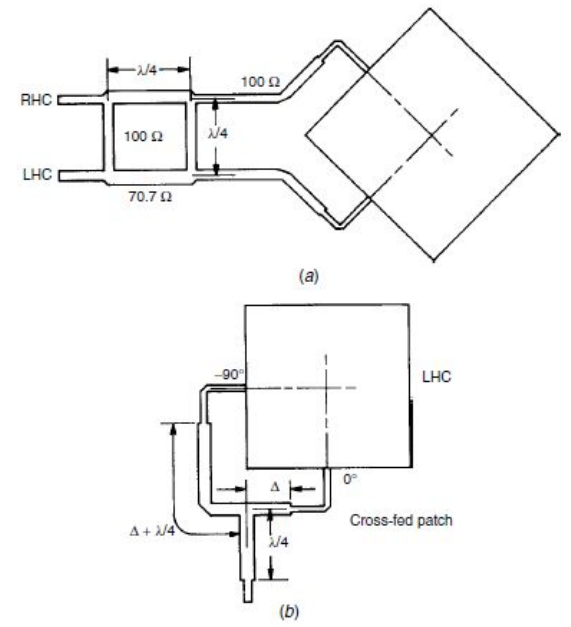
\includegraphics[width=.6\textwidth]{src/patch-antenna-circular-polarization.png}
        \caption{\label{fig:patch-antenna-circular-polarization}Feeding a microstrip antenna to produce a circular polarization}
    \end{figure}
    
    \item \emph{Frequency independent antennas -- self complementary antennas. By which dimensions are they specified?}
    
    \item \emph{Log-per antenna properties (directivity, bandwidth, phase center), compare to Yagi-Uda}
    
    \item \emph{Helix antenna modes and their radiation and impedance properties}
    
\end{enumerate}

\section{Characteristic modes}
\begin{enumerate}
    \item \emph{Antenna as an external resonator -- Characteristic modes (CM). Impedance matrix decomposition. Does CM depend on feeding? What happen with modes when you feed the antenna?}
    \item \emph{Physical properties of CM -- characteristic currents and eigenvalues, orthogonality, resonance}
    \item \emph{Are CM important for electrically small or large antennas?}
    \item \emph{Sketch first few modes on a electric dipole}
    \item \emph{Excitation of modes, importance of CM for design of mobile antennas}
\end{enumerate}

\section{Q factor}
\begin{enumerate}
    \item \emph{Definition of quality factor Q}
    \item \emph{Relation between Q and bandwidth of antenna.}
    \item \emph{Q factor and size of the antenna}
    \item \emph{Stored energy for antenna in frequency domain -- why is it infinite by definition?}
    \item \emph{Q factor from input impedance}
    \item \emph{Q factor for coupled structures, will it be higher for in- or out-of phase currents and why?}
    
    
    
    
\end{enumerate}

\end{document}